\documentclass[crop,tikz]{standalone}

\tikzset{>=latex}
\usetikzlibrary{decorations.markings}
\newcommand{\place}{\vec{r}}
\newcommand{\velocity}{\vec{v}}
\newcommand{\acceleration}{\vec{a}}

\begin{document}
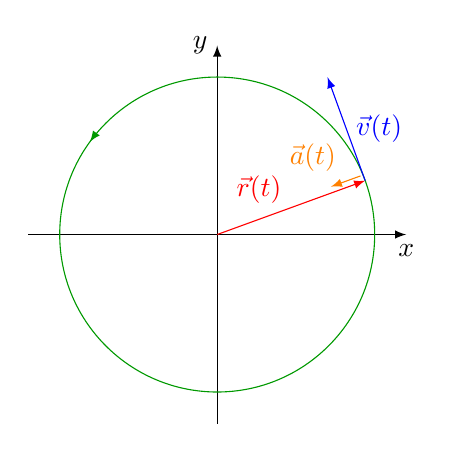
\begin{tikzpicture}[scale=2]
  % axes
  \draw[->] (-1.2,0) -- (1.2,0) node[below] {$x$};
  \draw[->] (0,-1.2) -- (0,1.2) node[left] {$y$};
  % circle
  \draw[
    decoration={markings, mark=at position 0.4 with {\arrow{>}}},
    postaction={decorate},
    black!40!green
  ] (0,0) circle (1);
  % place, velocity, acceleration
  \draw[->,red] (0,0) -- node[left,anchor=south east,yshift=-0.2em]{$\place(t)$} (20:1);
  \draw[->,blue] (20:1) -- node[right,anchor=west]{$\velocity(t)$} +(20+90:0.7);
  \begin{scope}[shift={(-0.03,0.03)}]
    \draw[->,orange] (20:1) -- node[left, anchor=south east] {$\acceleration(t)$} (20:0.8);
  \end{scope}
\end{tikzpicture}
\end{document}
